This test problem simulates an incident flux at a shallow angle to
the bottom edge of a 2-D void region.
This test reveals the diffusivity of a transport scheme in the transverse
direction; with some artificial diffusion, the ``sides'' of a radiation beam,
not just the front, will diffuse.
Table \ref{tab:glance_in_void} summarizes the problem parameters.

%-------------------------------------------------------------------------------
\begin{table}[htb]\caption{Glance in Void Test Problem Summary}
\label{tab:glance_in_void}
\centering
\begin{tabular}{l l}\toprule
\emph{Parameter} & \emph{Value}\\\midrule
Domain & $\mathcal{D} = (0,10)^2$\\
Initial Conditions & $u_0(\x)=0$\\
Boundary Conditions & $u(\x,t)=\left\{\begin{array}{c c}
  \frac{\pi}{3} & y = 0, \, t > 0\\
  0             & x = 0, \, t > 0
  \end{array}\right. \eqc$
Direction & $\mathbf{\Omega} = ()$\\
Cross Section & $\sigma(\x)=0$
Source & $q(\x,t)=0$\\
Speed & $\speed=1$\\
\bottomrule\end{tabular}
\end{table}
%-------------------------------------------------------------------------------

This test problem was run on a 64-cell$\times$64-cell mesh.

%with the time step
%size set equal to 


Table \ref{tab:void_to_absorber_run_parameters} shows the run parameters used
to obtain the results in this section, Figures \ref{fig:void_to_absorber_2D_fe}
and \ref{fig:void_to_absorber_2D_ssprk33} show 2-D results for explicit Euler
and SSPRK33 time discretizations, respectively, and Figure
\ref{fig:void_to_absorber_3D} shows 3-D results.

From Figure \ref{fig:void_to_absorber_2D_ssprk33}, one can see that the
Galerkin scheme (which has no artificial dissipation) generates significant
spurious oscillations perpindicular to the transport direction, even below the
absorber region. The oscillations are particularly severe along the lower edge
of the absorber region, where particles/photons are travelling parallel to the
absorber; this edge has a sharper gradient in the solution than the left edge
of the absorber region due to the lack of attenuation in this direction, which
is present for the left edge. Figure \ref{fig:void_to_absorber_2D_ssprk33},
which uses explicit Euler instead of SSPRK33 does not show the Galerkin plot
because the oscillations grew without bound, leading to infinite solution
values. The entropy viscosity scheme is also vulnerable to spurious
oscillations, although to a lesser extent than the Galerkin scheme.

%-------------------------------------------------------------------------------
\begin{table}[ht]\caption{Normal Void-to-Absorber Test Problem Run Parameters}
\label{tab:void_to_absorber_run_parameters}
\centering
\begin{tabular}{l l}\toprule
\emph{Parameter} & \emph{Value}\\\midrule
Number of Cells & $N_{cell} = 16384$\\
End Time & $t = 1$\\
CFL Number & $\nu = 0.5$\\\midrule
Entropy Function & $\entropy(\scalarsolution) = \frac{1}{2}\scalarsolution^2$\\
Entropy Residual Coefficient & $\entropyresidualcoef = 0.1$\\
Entropy Jump Coefficient & $\entropyjumpcoef = 0.1$\\
\bottomrule\end{tabular}
\end{table}
%-------------------------------------------------------------------------------
\begin{figure}[ht]
   \centering
   \begin{subfigure}{0.3\textwidth}
      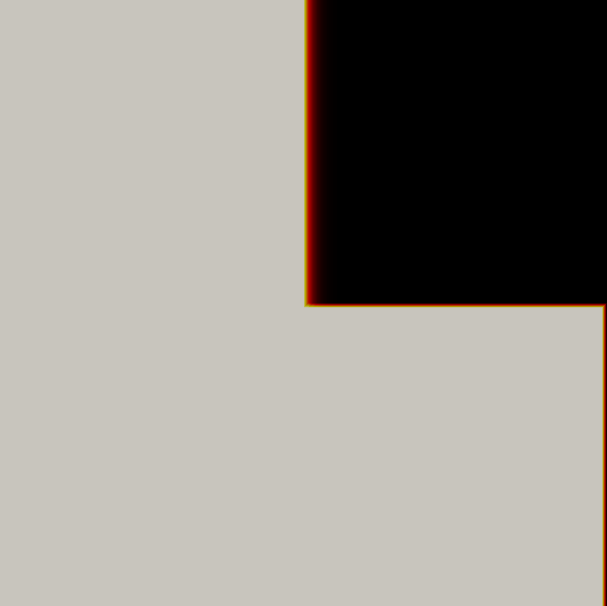
\includegraphics[width=\textwidth]
        {\contentdir/results/transport/void_to_absorber/images/Exact.png}
      \caption{Exact}
   \end{subfigure}
   \begin{subfigure}{0.3\textwidth}
      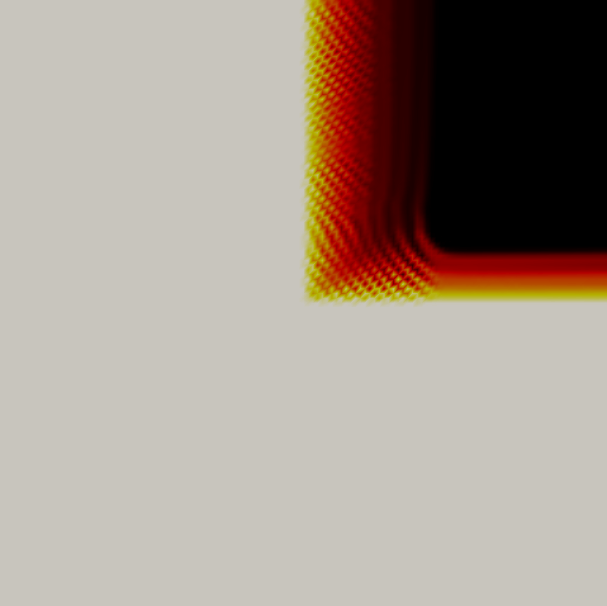
\includegraphics[width=\textwidth]
        {\contentdir/results/transport/void_to_absorber/images/GalFCT_FE.png}
      \caption{Galerkin FCT}
   \end{subfigure}
   \begin{subfigure}{0.3\textwidth}
      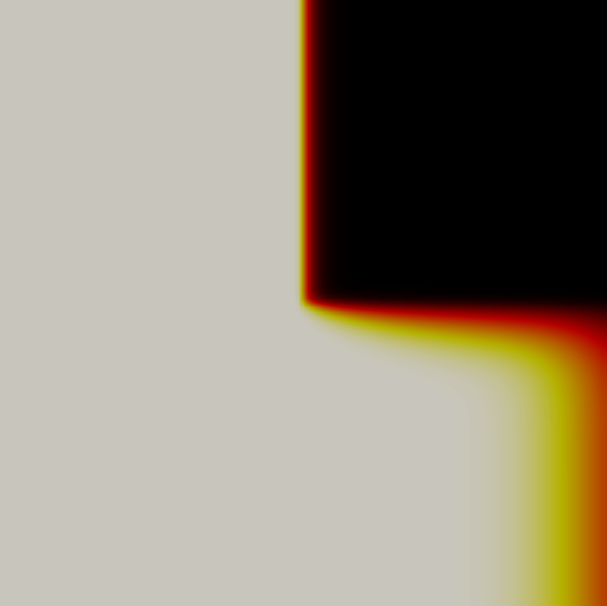
\includegraphics[width=\textwidth]
        {\contentdir/results/transport/void_to_absorber/images/Low_FE.png}
      \caption{Low-Order}
   \end{subfigure}
   \begin{subfigure}{0.3\textwidth}
      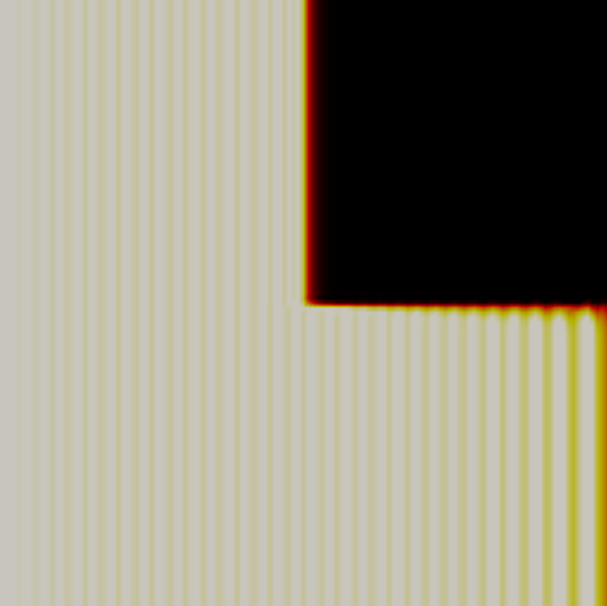
\includegraphics[width=\textwidth]
        {\contentdir/results/transport/void_to_absorber/images/EV_FE.png}
      \caption{Entropy Viscosity}
   \end{subfigure}
   \begin{subfigure}{0.3\textwidth}
      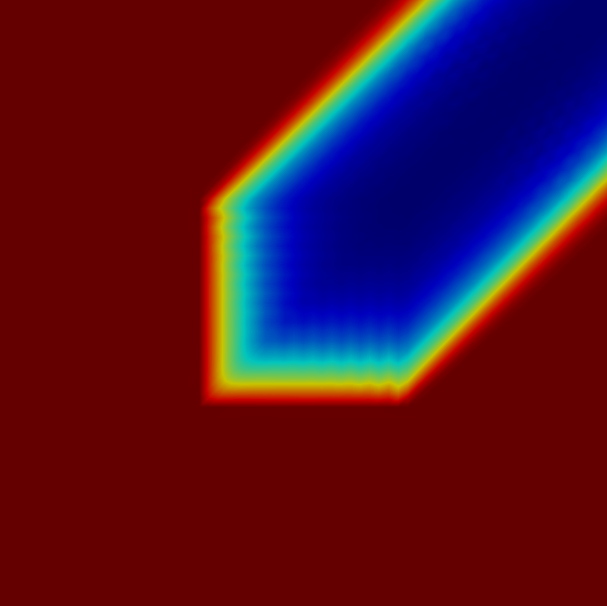
\includegraphics[width=\textwidth]
        {\contentdir/results/transport/void_to_absorber/images/EVFCT_FE.png}
      \caption{Entropy Viscosity FCT}
   \end{subfigure}
   \caption{Comparison of Solutions for 2-D Normal Void-to-Absorber Test
     Problem Using Explicit Euler Time Discretization}
   \label{fig:void_to_absorber_2D_fe}
\end{figure}
%-------------------------------------------------------------------------------
\begin{figure}[ht]
   \centering
   \begin{subfigure}{0.3\textwidth}
      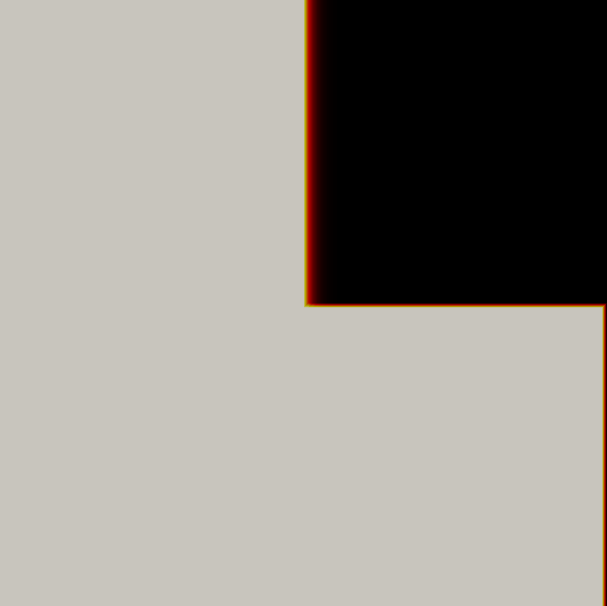
\includegraphics[width=\textwidth]
        {\contentdir/results/transport/void_to_absorber/images/Exact.png}
      \caption{Exact}
   \end{subfigure}
   \begin{subfigure}{0.3\textwidth}
      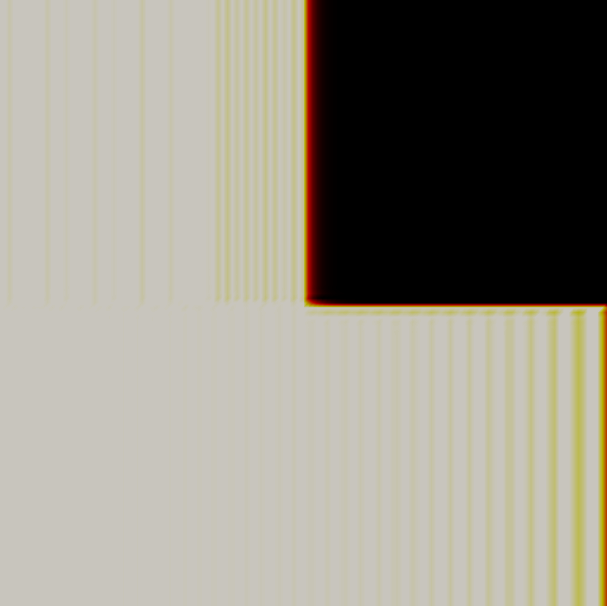
\includegraphics[width=\textwidth]
        {\contentdir/results/transport/void_to_absorber/images/Gal_SSPRK33.png}
      \caption{Galerkin}
   \end{subfigure}
   \begin{subfigure}{0.3\textwidth}
      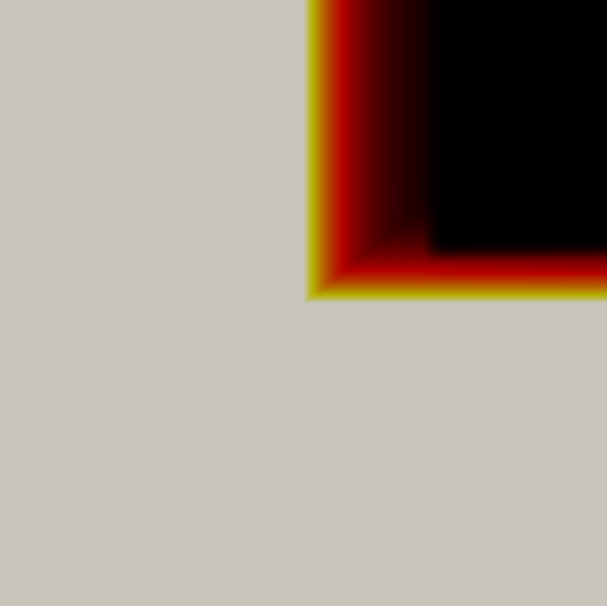
\includegraphics[width=\textwidth]
        {\contentdir/results/transport/void_to_absorber/images/GalFCT_SSPRK33.png}
      \caption{Galerkin FCT}
   \end{subfigure}
   \begin{subfigure}{0.3\textwidth}
      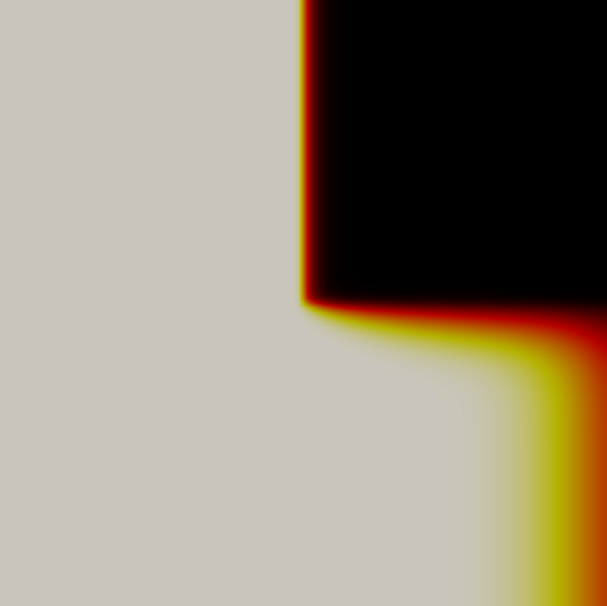
\includegraphics[width=\textwidth]
        {\contentdir/results/transport/void_to_absorber/images/Low_SSPRK33.png}
      \caption{Low-Order}
   \end{subfigure}
   \begin{subfigure}{0.3\textwidth}
      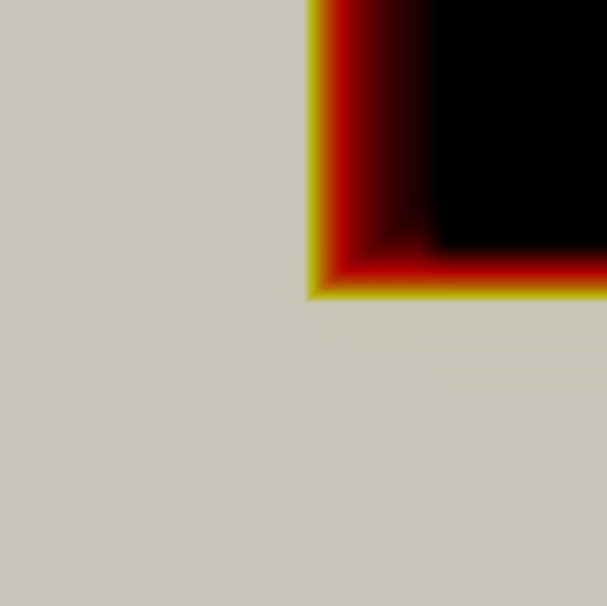
\includegraphics[width=\textwidth]
        {\contentdir/results/transport/void_to_absorber/images/EV_SSPRK33.png}
      \caption{Entropy Viscosity}
   \end{subfigure}
   \begin{subfigure}{0.3\textwidth}
      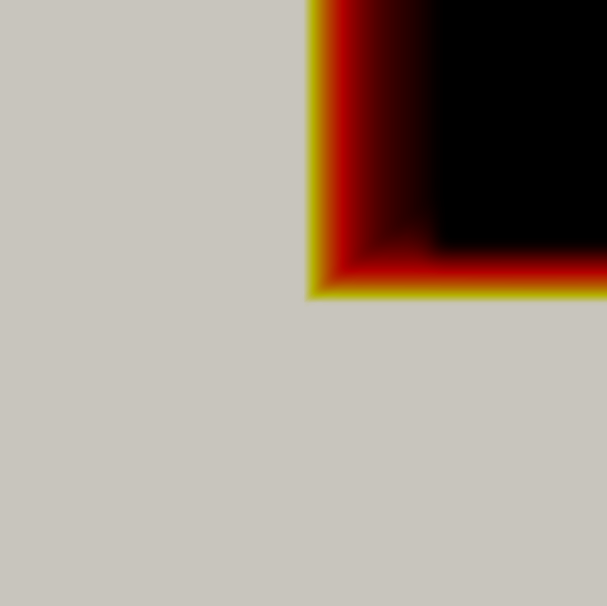
\includegraphics[width=\textwidth]
        {\contentdir/results/transport/void_to_absorber/images/EVFCT_SSPRK33.png}
      \caption{Entropy Viscosity FCT}
   \end{subfigure}
   \caption{Comparison of Solutions for 2-D Normal Void-to-Absorber Test
     Problem Using SSPRK33 Time Discretization}
   \label{fig:void_to_absorber_2D_ssprk33}
\end{figure}
%-------------------------------------------------------------------------------
\begin{figure}[ht]
   \centering
   \begin{subfigure}{0.45\textwidth}
      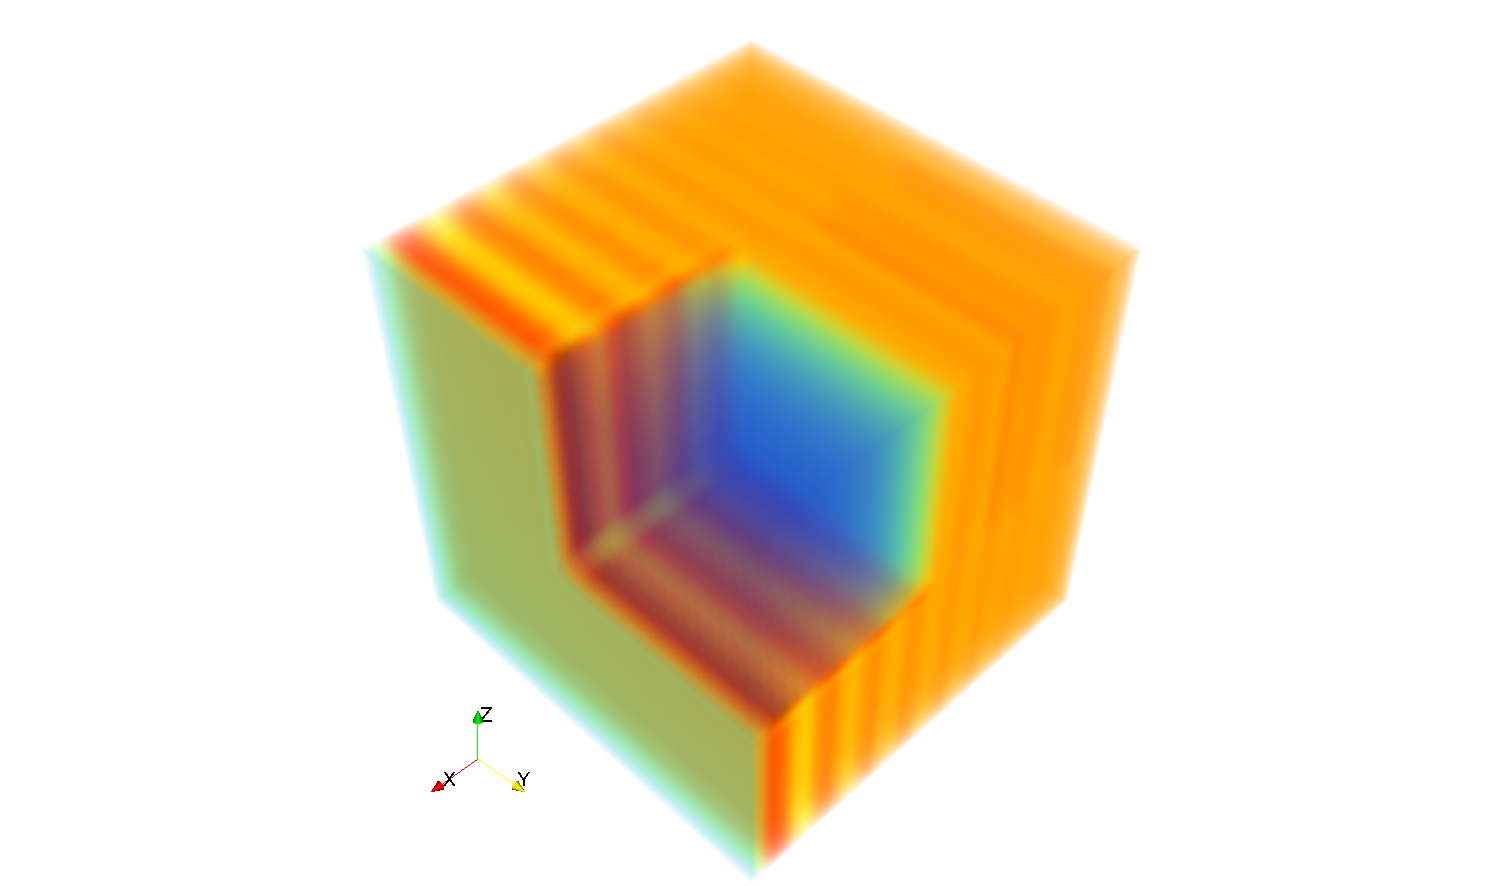
\includegraphics[width=\textwidth]
        {\contentdir/results/transport/void_to_absorber/images/Gal_3D.png}
      \caption{Galerkin}
   \end{subfigure}
   \begin{subfigure}{0.45\textwidth}
      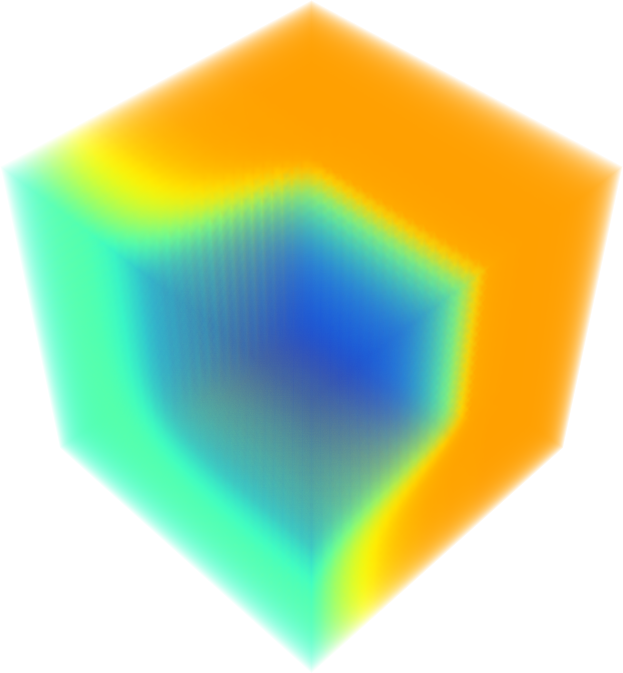
\includegraphics[width=\textwidth]
        {\contentdir/results/transport/void_to_absorber/images/GalFCT_3D.png}
      \caption{Galerkin with FCT}
   \end{subfigure}
   \caption{Comparison of Solutions for the 3-D Normal Void-to-Absorber Test
     Problem Using SSPRK33 Time Discretization}
   \label{fig:void_to_absorber_3D}
\end{figure}
%-------------------------------------------------------------------------------

\clearpage
